%!TEX root=main.tex
\section{系统实现}
\label{clicknp:sec:impl}

\subsection{\name 工具链与硬件平台}

本章实现了一个\name 编译器,作为\name 工具链的前端(\S \ref {clicknp:subsec:toolchain})。
对于宿主程序,使用Visual C++作为后端。进一步集成了 Altera OpenCL SDK(即 Intel FPGA SDK for OpenCL) \cite {aoc} 和 Xilinx SDAccel \cite {vivado}作为FPGA程序的后端。
\name 编译器包含约 2 万行 C++、flex 和 bison 代码,它们解析配置文件和元件声明,执行第 \ref {clicknp:sec:optimization} 节所述的优化,并生成特定于每个商业高层次综合工具的代码。

对于在 FPGA 上运行的元件,每个元件被编译成中间 C 代码,进而通过高层次综合工具编译成一个逻辑模块。
使用 Altera OpenCL 高层次综合工具时,每个 \name 元件都被编译成 \textit {kernel},元件之间的连接被编译为Altera 扩展通道(channel),进而用 Avalon ST 接口实现;元件与板上 DRAM(即全局内存)之间使用 Avalon MM 接口通信。
使用 Xilinx SDAccel 高层次综合工具时,将每个元件编译成IP核(IP core),并使用AXI流(stream)来实现元件之间的连接,实现AXI内存映射接口访问板上DRAM。
在主机上运行的元件被编译为CPU二进制文件,管理进程将为每个主机元件创建一个工作线程。
主机和FPGA元件之间的每条管道都映射到PCIe I/O通道的\textit {插槽}(\S \ref {clicknp:subsec:pcie})。

本文的硬件平台基于Altera Stratix V FPGA和Catapult shell \cite {putnam2014reconfigurable}。
Catapult shell还包含一个OpenCL特定的运行时(BSP)。\name 用户逻辑通过 BSP 与shell通信。
\name 用户逻辑运行在独立的时钟域内,BSP 将 shell 中处于不同时钟域的 PCIe DMA、DRAM 等接口通过异步 FIFO 转换为用户逻辑所在的时钟域。
BSP 还提供了 OpenCL 内核启动、停止等管理功能。
撰写本文时,作者还没有获得Xilinx硬件平台。
因此,系统评估主要基于使用\name + OpenCL的Altera平台,使用Vivado HLS生成的报告(例如频率和面积成本)来了解\name + Vivado的性能。


\subsubsection{适合高层次综合工具的中间 C 代码}

当主机上电或 FPGA 被在线重配置后,各个 kernel 或 IP 核就开始并行运行。如图 \ref{clicknp:fig:intermediate-c} 所示,每个 kernel 首先执行初始化(init)函数,然后进入永不退出的循环,检查输入管道并执行事件处理(handler)函数,检查信号并执行事件处理函数。

\begin{figure}[htbp]
	\small
	\centering
	\begin{tabular}{c}
\begin{lstlisting}
void kernel() {
  调用 init 函数;
  声明并初始化输入输出缓冲区;
  while (true) {
    if (输入缓冲区有空闲 and 输入管道非空) {
      从输入管道中搬移数据到输入缓冲区;
    }
    调用 handler 函数;
    if (输出管道有空闲 or 输出缓冲区已满) {
      从输出缓冲区搬移数据到输出管道;
    }
    if (输入事件管道非空) {
      从输入事件管道读取输入事件;
      调用 signal 函数;
      将事件处理响应写入输出事件管道;
    }
  }
}
\end{lstlisting}
	\end{tabular}
	\caption{Kernel 中间 C 代码的伪代码。}
	\label{clicknp:fig:intermediate-c}
\end{figure}

高层次综合工具将中间 C 代码变换成硬件描述语言,中间 C 代码中的每层循环或者被完全展开(unroll)成流水线化的逻辑模块,或者被实现成状态机,每个时钟周期执行循环的一次迭代。循环展开仅适用于循环次数在编译时静态可知,且循环次数较小的情况。对于实现成状态机的循环,由于循环的各次迭代之间可能存在数据依赖,且一次迭代的流水线逻辑可能需要若干个时钟周期才能执行完毕,相邻两次循环迭代间可能需要若干时钟周期的间隔。高层次综合工具需要根据依赖关系和循环体的流水线延迟信息,计算相邻两次迭代的最小间隔(initiation interval,II)。II 越小,吞吐量越高。因此,我们希望尽量减小 II。

目前,高层次综合工具为计算密集型操作设计。计算密集型操作往往由多层嵌套循环构成,编译器使用的循环变换方法通常适用于控制流编译时静态可知(static control part)、完美嵌套循环(perfectly nested loop)的程序。然而,图 \ref{clicknp:fig:intermediate-c} 的程序中 while 循环的执行次数在编译时不可知,且由于输入输出缓冲区搬移代码的存在,handler 和 signal 函数中的循环均不是完美嵌套循环。早期版本的高层次综合工具由于完备性问题,不仅对较为复杂的源程序可能出现编译失败、编译时间过长等错误,还可能分析出过多不必要的内存依赖,导致 II 过大,甚至导致 II 静态分析失败,内层循环无法并行。

本文希望绕过现有高层次综合工具的嵌套循环优化。注意到网络功能中的元件计算逻辑相对简单,每个时钟周期处理的数据量也很有限(如一个 flit),很多循环的执行次数可以在编译时静态确定(例如处理一个 flit 的每个字节)。因此,\name 将 handler 和 signal 函数中的所有循环进行展开(unroll)或压平(flatten),使生成的中间 C 代码仅有 while 一层循环,而不再有嵌套循环,如图 \ref{clicknp:fig:flatten} 所示。\name 的默认策略是展开循环次数可在编译时确定的循环,并压平所有其他循环。用户也可以通过嵌入在源程序中的编译选项(pragma)指定展开和压平的策略。这样,高层次综合工具只需分析单层循环,减小了出错的可能性。展开循环体还有一个重要的好处:便于编译优化。传统编译器往往很难优化用循环表示的向量操作,但 \name 进行循环展开后向量操作被分解为逐点操作,高层次综合工具就可以进行常量传播、死代码消除等一系列优化,并将每个点的操作映射到 FPGA 上的逻辑门。

\name 可以生成性能分析报告。在每个元件内,分析报告包括每个变量的存储方式,每个循环的展开或压平策略,相邻两次迭代的最小间隔(II)以及导致 II 瓶颈的依赖关系链。在计算图层次上,分析报告包括每个元件的延迟、吞吐量和时钟频率。

\begin{figure}
	\lstset{style=numbers}
	
	\centering
	\renewcommand{\baselinestretch}{0.75}
	\begin{tabular}{c}
		{
			\small
\begin{lstlisting}[escapechar=@]
while (true) {
  Packet pkt = read_input_port(in);
  uchar checksum = 0;
  #pragma unroll 2
  for (int i = 0; i < pkt.num_flits(); i++) {
    flit f = pkt.filt(i);
    for (int j = 0; j < FLIT_BYTES; j++)
      checksum ^= f.bytes[j];
  }
  write_output_port(out, checksum);
}
\end{lstlisting} 
		} \\
		(a) 原始的 C 中间代码(示意代码)。  \\
		{
			\small 
\begin{lstlisting}[escapechar=@]
uchar checksum = 0;
Packet pkt;
int i = 0;
while (true) {
  if (i == 0)
    pkt = read_input_port(in);
  if (i < pkt.num_flits()) {
    flit f = pkt.filt(i);
    checksum ^= f.bytes[0]; checksum ^= f.bytes[1];
    ...
    checksum ^= f.bytes[FLIT_BYTES - 1];
    i++;
  }
  if (i < pkt.num_flits()) {
    flit f = pkt.filt(i);
    checksum ^= f.bytes[0]; checksum ^= f.bytes[1];
    ...
    checksum ^= f.bytes[FLIT_BYTES - 1];
    i++;
  }
  if (i == pkt.num_flits()) {
    write_output_port(out, checksum);
    i = 0;
  }
}
\end{lstlisting} 
		} \\
		(b) 循环展开和压平后的结果。
	\end{tabular}
	\caption{循环展开和压平。对 i 循环按照并行度 2 进行展开,并压平;j 循环完全展开:变换的结果是每个时钟周期计算 2 个 flit 的所有字节。}
	\label{clicknp:fig:flatten}
\end{figure}

\subsubsection{编译速度优化}

FPGA 编程的一个限制是编译时间相当长。一个网络数据包简单转发的功能就需要 3 小时来编译。编译时间主要由高层次综合、IP 核生成、硬件描述语言逻辑综合、FPGA 布局布线、时序分析等几个阶段构成。
本章采用几项技术来缩短 FPGA 编译时间。
第一,OpenCL 编程框架会把高层次综合生成的 Verilog 模块生成 IP 核,插入到 shell 部分中,这需要复制大量 IP 核和 shell 部分的代码。注意到用户逻辑的外围接口是固定的,本文预先生成 IP 核,只需将高层次综合 Verilog 模块文件替换进项目中;对于 shell 部分代码,使用文件引用而非拷贝。
第二,为了缩短逻辑综合时间,将固定的 shell 部分通过逻辑综合生成网表(netlist)文件,利用设计分区(design partition)保留综合结果,可以将 shell 部分的逻辑综合时间减少约 35 分钟。
第三,为了加快 FPGA 布局算法的收敛速度,在初始编译完成后,增加 shell 部分各模块的布局约束,将其布局基本上固定下来。shell 部分的模块大多与芯片固定位置的硬核(hard IP)交互,固定布局在硬核附近是合理的。但是为了更好的性能,本文没有使用设计分区将 shell 部分的布局布线完全固定下来。这项优化可节约大约 20 分钟。
第四,区分调试(debug)和发布(release)编译模式。调试模式旨在验证逻辑上的正确性,而不追求性能。在调试模式下,把用户逻辑的时钟频率固定为 50~MHz,大大降低了布局布线的难度;使用设计分区固化 shell 部分的布局布线,这部分高频逻辑的布局布线需要较长的时间。调试模式相比发布模式可节约 25 分钟编译时间,在用户逻辑更复杂时节约的时间将更多。
第五,删除不必要的时序分析模型。OpenCL 框架默认在四种情形下分析时序约束,但只要满足其中最苛刻的一种,其余三种也能满足,因此我们仅保留最苛刻的时序约束模型。
第六,OpenCL 框架为了尽可能提高性能,首先使用较高的用户逻辑时钟频率(如 250~MHz)编译,然后根据时序分析结果计算出最长延迟和能正确工作的最高时钟频率,再用该时钟频率进行二次布局布线和时序分析。这对计算密集型工作负载可以达到尽可能高的吞吐量。然而,本文关注网络数据包处理,只需达到网络线速的处理能力,因此可以固定时钟频率为 180 MHz,大多数用户逻辑均可达到此频率,因此无需重新布局布线。

\begin{table}[htbp]
	\centering
	\caption{FPGA 编译加速技术。}
	\label{clicknp:tab:fpga-compilation}
	\small
	\begin{tabular}{l|p{.4\textwidth}|p{.15\textwidth}|p{.15\textwidth}}
		\toprule
		编译阶段 & 优化方法 & 优化前编译时间(分) & 优化后编译时间(分) \\
		\midrule
		ClickNP 编译 & -- & 0.1 & 0.1 \\
		高层次综合 & -- & 1 & 1 \\
		生成 IP 核 & 预先生成 IP 核;使用文件引用而非拷贝 & 10 & 0 \\
		逻辑综合 & 保留 shell 的综合结果 & 50 & 15 \\
		布局布线 & 增加 shell 的布局约束;调试模式下降低用户逻辑的时钟频率,保留 shell 的布局布线结果 & 60 & 40 (15)* \\
		时序分析 & 删除不必要的时序分析模型 & 15 & 5 (0)* \\
		二次布局布线 & 固定时钟频率,无需重新布局布线 & 30 & 0 \\
		二次时序分析 & 删除 & 15 & 0 \\
		\midrule
		总计 & -- & 180 & 60 (30)* \\
		\bottomrule
		\multicolumn{4}{l}{* 括号内是调试模式下的编译时间。}
	\end{tabular}
\end{table}

表 \ref{clicknp:tab:fpga-compilation} 总结了上述编译加速技术。优化前,开发者每个工作日只能进行 3 轮调试,而优化后在调试模式下可调试 10 轮左右,需要性能的系统测试也可进行约 6 轮,大大提高了工作效率。


\subsection{\name 元件库}
\label{clicknp:subsec:lib}

本文实现了一个包含近 200 个元件的 \name{} 元件库。
其中一部分(约20%)直接来自Click Modular Router,但使用 \name{} 编程框架重新编写。
这些元件涵盖了网络功能的大量基本操作,包括数据包解析,校验和计算,封装/解封,哈希表,最长前缀匹配(LPM),速率限制,加密和数据包调度。
由于\name 有模块化的体系结构,每个元件的代码大小都是适中的。
元件的平均代码行数(Line of Code,LoC)是80,最复杂的元件 \textit {PacketBuffer} 有196行C代码\footnote{代码行数是指 ClickNP 元件代码,不包括主机控制程序和测试代码。}。


\begin{sidewaystable}[htbp]
	\centering
	\caption{\name 中的一些网络元件。}
	\label{clicknp:tab:elements}
	\small
	\begin{tabular}{l|l|l|l|l|l|l|r|r}
		\toprule
		&	&	& \multicolumn{4}{c|}{性能} & \multicolumn{2}{c}{资源占用 (\%)} 			\\
		\cline{4-7} \cline{8-9}  
		
		元件 	& 配置 & 优化 & \tabincell{c}{最高频率\\ (MHz)} & 峰值吞吐量 & 加速比 (FPGA/CPU) & 延迟(时钟周期) & LE & BRAM \\
		\midrule
		L4\_Parser (A1-5)  & N/A & REG & 221.93 & 113.6 Gbps & 31.2x / 41.8x & 11 & 0.8\% & 0.2\% \\
		IPChecksum (A1-4) & N/A & UL & 226.8 & 116.1 Gbps & 33.1x / 55.1x & 18 & 2.3\% & 1.3\% \\
		NVGRE\_Encap (A1,4) & N/A & REG, UL & 221.8 & 113.6 Gbps & 35.5x / 42.9x & 9 & 1.5\% & 0.6\% \\
		\midrule
		AES\_CTR (A3) & 16 字节块大小 & UL & 217.0 & 27.8 Gbps & 79.9x / 255x & 70 & 4.0\% & 23.1\% \\
		SHA1 (A3) & 64B 字节块大小 & MS, UL & 220.8 & 113.0 Gbps & 157.5x / 83.1x & 105 & 7.9\% & 6.6\% \\
		\midrule
		\midrule
		CuckooHash (A2) & 128K 个条目 & MS, UL, DW & 209.7 & 209.7 Mpps & 43.6x / 57.5x & 38 & 2.0\% & 65.5\% \\
		HashTCAM (A2) & 16 x 1K 个条目 & MS, UL, DW & 207.4 & 207.4 Mpps & 155.9x / 696x & 48 & 18.7\% & 22.0\% \\
		LPM\_Tree (A2) & 16K 个条目 & MS, UL, DW & 221.8 & 221.8 Mpps & 34.5x / 45.2x & 181 & 4.3\% & 13.2\% \\
		FlowCache (A4) & 4 路组相连,16K 条目 & MS, DW & 105.6 & 105.6 Mpps & 55.8x / 21.5x & 27 & 5.6\% & 46.9\% \\
		\midrule
		
		SRPrioQueue (A5) & 32 个数据包的缓冲区 & REG, UL & 214.5 & 214.5 Mpps & 150.3x / 28.6x & 41 & 2.6\% & 0.6\% \\
		RateLimiter (A1,5) & 16K flows & MS, DW & 141.5 & 141.5 Mpps & 7.0x / 65.3x & 14 & 16.9\% & 14.1\% \\
		\bottomrule
		
		\multicolumn{9}{l} {\textbf{优化方法。} REG=Using Registers 使用寄存器; MS=Memory Scattering 内存散射; UL=Unroll Loop 循环展开; DW=Delay Write 延迟写入。} \\
		\multicolumn{9}{l} {\parbox{\textwidth}{\textbf{性能提升} 一列对比了应用第 \S\ref{clicknp:sec:optimization}  节的优化后和优化前的 FPGA 性能。也列出了与 CPU 实现间的性能对比。}}
		
	\end{tabular} 
\end{sidewaystable}

表 \ref {clicknp:tab:elements} 显示了在 \name 中实现的一组选定的关键元件。
除了元件名称,还标记了使用该元件的演示网络功能(在 \S \ref {clicknp:sec:application} 中讨论)。
之前在 \S \ref {clicknp:subsec:paral_in_elem} 中讨论的优化技术最小化了内存依赖性,并平衡了流水线阶段。
第3列总结了每个元件使用的优化技术。
对于表 \ref {clicknp:tab:elements} 顶部的元件,元件中的处理逻辑需要访问数据包的每个字节。其中吞吐量以Gbps显示。
但是,表格底部的元件只处理数据包头(元数据)。因此,使用每秒数据包来测量吞吐量更有意义。
值得注意的是,表 \ref {clicknp:tab:elements} 中测量的吞吐量是相应元件可以实现的最大吞吐量。
当它们在真正的网络功能中工作时,其他组件,例如以太网端口,可能是瓶颈。
作为参考,表 \ref {clicknp:tab:elements} 比较了优化后的 FPGA 版本、不应用 \S\ref {clicknp:sec:optimization} 所述技术的 FPGA 简单实现以及 CPU 实现。
很明显,经过优化后,所有这些元件都可以非常高效地处理数据包,与初始的FPGA实现相比,速度提高了7至117倍,与一个CPU内核上的软件实现相比,速度提高了21%。
这种性能提升来自于利用FPGA中的巨大并行性的能力。
考虑到FPGA的功耗(大约30W)和CPU(每个核心大约5W),\name 元件的能耗效率比CPU高4到120倍。

表 \ref {clicknp:tab:elements} 还显示了每个元件的处理延迟。
可以看到,这个延迟很低:平均值是 $0.19 \mu s$,最大值仅为$0.8 \mu s$(LPM \_Tree)。
最后两列总结了每个元件的资源利用率。 利用率归一化为FPGA芯片的容量。
大多数元件只使用少量的逻辑元件。
这是合理的,因为大多数数据包操作都很简单。
HashTCAM和RateLimiter具有适度的逻辑资源使用,因为这些元件具有更大的仲裁逻辑。
但是,BRAM的使用很大程度上依赖于元件的配置。 例如,BRAM使用率随流表中支持的条目数呈线性增长。
总而言之,本文使用的FPGA芯片有足够的容量来支持包含少量元件的有意义的网络功能。


\subsection{PCIE I/O 通道}
\label{clicknp:subsec:pcie}

如前所述,\name 的一个关键属性是支持联合CPU / FPGA处理。
本章通过设计高吞吐量,低延迟的PCIe I / O通道来实现这一目标。
\name 支持灵活的 I/O 操作。如图 \ref{clicknp:fig:pcie-io} 所示,\name 提供了基于槽位(slot)和工作队列(work queue)两种与主机 CPU 通信的抽象,还提供了裸 DMA 操作的接口。


\begin{figure}[htbp]
	\centering
	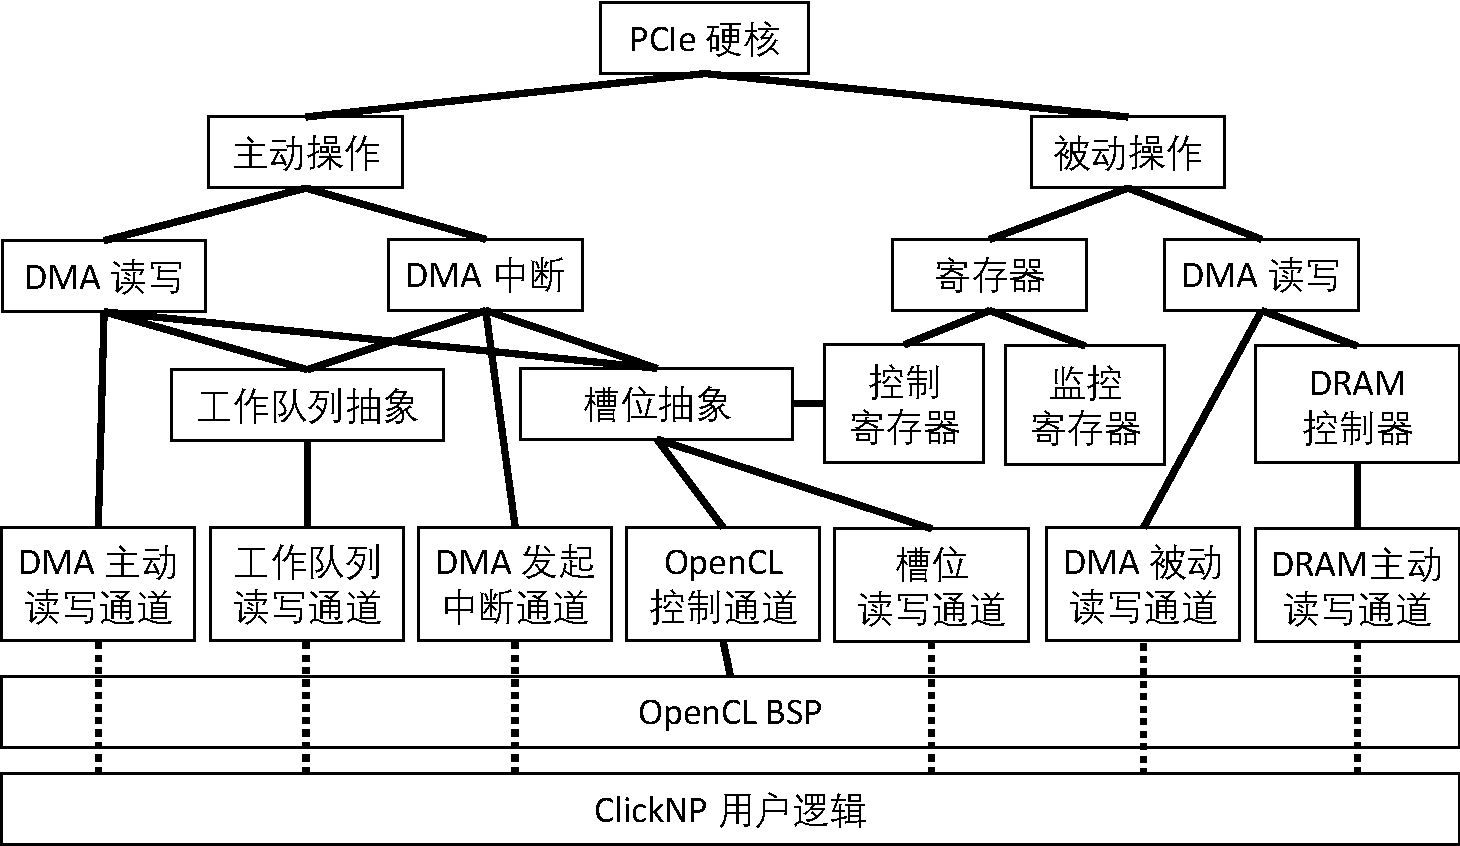
\includegraphics[width=0.8\textwidth]{image/pcie-io}
	\caption{PCIe I/O 通道的架构。}
	\label{clicknp:fig:pcie-io}
\end{figure}


在基于槽位的抽象中,PCIe 物理链路划分为64个逻辑子通道,即\textit {slots}(插槽)。
每个插槽都有一对用于DMA操作的发送和接收缓冲区。
在64个插槽中,33个由 OpenCL BSP 用于管理 ClickNP 内核和访问板载 DDR(即 OpenCL 控制通道),一个插槽用于将信号传递给 \name 元件。
剩余的30个插槽用于FPGA和CPU元件之间的数据通信。
CPU 上的槽位抽象可以在中断或轮询模式下工作。

槽位抽象中每发送一个数据都需要至少 4 次 DMA 操作 \footnote{从主机 CPU 发送数据到 FPGA 的过程是:主机 CPU 写 FPGA 中的下行控制寄存器(又称门铃,doorbell);FPGA 从主机内存中 DMA 读取数据。当 FPGA 处理完槽位中的数据后,写主机内存中的下行完成寄存器,并向主机 CPU 发送中断。从 FPGA 向主机 CPU 发送数据的过程是:FPGA 读内部的上行控制寄存器,判断为空;FPGA 向主机内存 DMA 写入数据,并向主机 CPU 发送中断。主机接收 FPGA 发来的数据过程是:读 FPGA 中的上行控制寄存器,判断非空;读取主机内存中的数据;写 FPGA 中的上行控制寄存器,表示处理完毕。},且需要等待对面的设备处理完成才能在同一槽位发送下一个数据。
为分摊 DMA 开销、提高消息发送的并发度,工作队列是槽位抽象的扩展,每个槽位不再仅有一对缓冲区,而是有一对用于发送和接收的环形缓冲区队列。
每条环形缓冲区队列有 128 个槽位,按照先进先出的方式访问。
发送端发现环形缓冲区队列中还有尚未被取走的数据时,就无需通知对端,节约了 CPU 通过 PCIe MMIO 发送门铃(doorbell)和 FPGA 发送中断的开销。

除了槽位和工作队列,FPGA 和 CPU 之间还需要更灵活的通信方式。首先,第 \ref{chapter:kvdirect} 章的键值存储中,FPGA 需要直接读写主机内存中的键值,而无需主机 CPU 参与,这就需要 FPGA 能够直接发出裸的 PCIe DMA 读写请求。
其次,在基于可编程网卡的内存解聚中,FPGA 将远程内存通过 PCIe MMIO 直接映射到主机内存空间,主机 CPU 直接访问此内存空间,生成 PCIe DMA 读写请求发送到 FPGA。FPGA 中的用户逻辑需要处理这些 DMA 被动读写操作。
最后,一些应用(如传统 OpenCL 应用)可能希望主机 CPU 与 FPGA 之间采用 FPGA 板上的 DRAM 作为共享内存,因此 FPGA 板上的 DRAM 通过 PCIe MMIO 映射到主机内存空间,由 shell 中的 PCIe 被动读写逻辑发送到 DRAM 控制器。由于主机 PCIe MMIO 读写大块数据的效率较低,也支持主机 CPU 通过控制寄存器,让 FPGA shell 主动发起 DMA 在板上 DRAM 和主机内存间搬运数据。



图 \ref {clicknp:fig:pcie} 显示了具有不同插槽数和批量大小的PCIe I/O通道的基准测试结果。
作为基线,还测量了OpenCL全局内存(global memory)操作的性能 -- 到目前为止,这是OpenCL \cite {opencl} 中CPU与FPGA间通信提供的唯一方法。
在图 \ref {clicknp:fig:pcie} 中可以看到,单个插槽的最大吞吐量约为8.4~Gbps。
通过4个插槽,PCIe I/O通道的总吞吐量可达25.6~Gbps \footnote{这是本章写作时使用的 PCIe Gen2 x8 硬核的实际最高性能。事实上该 FPGA 支持 PCIe Gen3 x8 硬核,第 \ref{chapter:kvdirect} 章通过替换硬核和优化 shell,实现了 2 倍的 PCIe I/O 通道吞吐量。}。
但是,OpenCL的吞吐量低得惊人,甚至低于1~Gbps。这是因为全局内存API旨在传输 GB 级的大量数据。这可能适用于具有大数据集的应用程序,但不适用于需要强流处理(stream prpocessing)功能的网络功能。
同样,图 \ref {clicknp:fig:pcie}(b)显示了通信延迟。由于OpenCL未针对流处理进行优化,因此OpenCL延迟高达1~ms,通常是网络功能无法接受的。
相比之下,PCIe I/O 通道在轮询模式下具有非常低的 1 $\mu$s 的延迟(一个 CPU 核持续轮询状态寄存器),而在中断模式下的延迟为 9 $\mu$s(几乎没有CPU开销) 。

\begin{figure}[htbp]
	\centering
	\subfloat[]{
		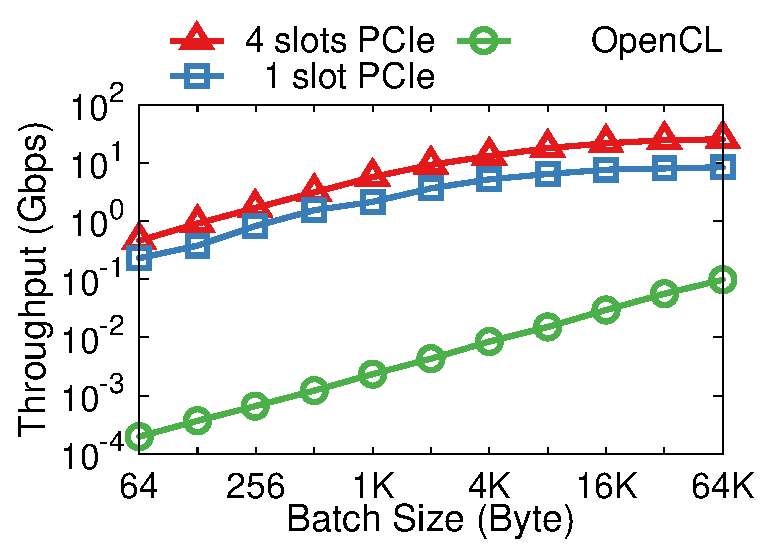
\includegraphics[width=0.5\textwidth]{eval/pcie_1}
	}
	\subfloat[]{
		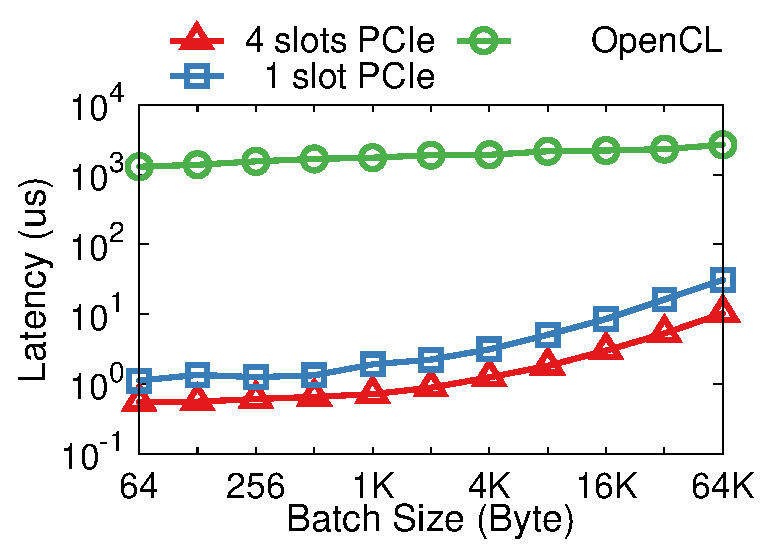
\includegraphics[width=0.5\textwidth]{eval/pcie_2}
	}

	\caption{PCIe I/O 通道的性能。Y 轴是对数坐标系。}

	\label{clicknp:fig:pcie}
\end{figure}

为了给 FPGA 元件发送信号,\name 编译器自动在 FPGA 中生成一个名为\textit {CmdHub} 的特殊元件。
\textit {CmdHub} 将主机管理程序下发的控制信号通过管道分发到FPGA元件,FPGA元件再将信号处理函数的结果通过管道返回给 \textit {CmdHub},进而返回给主机管理程序。
为了避免一对多管道连接带来的布局布线困难,\textit {CmdHub} 与所有元件构成一条菊花链,从 CmdHub 开始,按照元件连接图的拓扑排序依次穿过所有元件,最后回到 CmdHub。
为了在菊花链中识别目标元件,信号消息中嵌入了元件ID,每个元件仅处理匹配元件 ID 的信号消息,而对其他信号消息直接转发。
 


\subsection{调试}
\label{clicknp:subsec:debug}

\name 提供两种方法用于调试。

\textbf{CPU 功能仿真。}
\name 元件使用类 C 的高级语言编写,因此一个元件可以编译成 CPU 上运行的一个线程,而管道就是线程之间的队列。开发者可以使用熟悉的软件调试工具进行功能仿真。



\textbf{实际 FPGA 运行。}
CPU 功能仿真存在局限。首先,元件之间的通信管道有死锁的可能,在 CPU 功能仿真时由于时序与硬件逻辑不一致,不一定能发现死锁问题;其次,CPU 仿真速度较慢,不能反映实际性能,且难以测试与 PCIe DMA、网络之间的交互;最后,功能仿真不能发现编译器中的错误。为此,实际应用在功能仿真通过后,一般用实际 FPGA 运行的方法调试。

由于 \name 语言中的变量名与 Verilog 中的不匹配,SignalTap 等用于 FPGA 在线调试的工具并不适用。因此,\name 需要定制的调试机制。首先,在调试模式下,\name 可以记录每条管道的输入输出日志,并通过 PCIe I/O 管道传输到主机内存上。第二,\name 允许用户在元件代码中插入 printf 语句,通过管道将包含变量值的调试信息发送到主机端。第三,\name 支持用户在编译时插入断点,以便调试交互式网络协议或模拟队列阻塞导致的死锁。断点被编译成管道的写操作(通知主机断点命中)和阻塞读操作(等待主机发送断点继续命令)。第四,\name 允许在运行过程中(包括断点命中时)随时查询或修改某个变量的值。当用户查询某个变量的值时,通过 signal 发送查询或修改命令,并返回变量的值。

\subsection{元件热迁移和高可用}
\label{subsec:clicknp:fault-tolerance}

热迁移是数据中心网络功能需要支持的重要特性。当虚拟机热迁移时,计算节点对应的网卡内部状态需要热迁移到新节点,不然就需要在新节点上重新初始化网卡状态,带来软件的复杂性和迁移延迟。类似的,当网络、存储节点因升级、扩容等进行热迁移时,网卡状态也需要热迁移到新节点。此外,为了实现服务不间断的网络功能升级,需要将内部状态热迁移到另一节点,再将原节点下线进行升级。为了实现高可用性,当增加备份节点时,为了同步源节点和新增备份节点的内部状态,也需要热迁移技术。

当热迁移开始时,首先在交换机上进行配置,停止向旧 FPGA 发送数据包,而是将这些数据包缓冲在交换机内。然后通过第 \ref{clicknp:subsec:debug} 节的断点机制停止 FPGA 内各元件的运行,再将所有元件内变量的值、管道内的数据和全局内存的值导出到主机。接下来,在新 FPGA 上运行相同的 \name 程序,通过调试机制导入上述 FPGA 内部状态,并恢复各元件运行。最后,通知交换机修改路由表,将旧 FPGA 的地址指向新 FPGA 所在端口,发送交换机内缓冲的数据包,热迁移结束。

为了实现网络功能的高可用,\name 采用状态机复制的方法。两个 FPGA 接收到相同的数据包序列,只要元件内部没有随机化或与时间相关的处理逻辑,也不接受主机的控制信号,就能保证两个 FPGA 的内部状态和发出的数据包序列相同。当检测到备份节点故障时,只需启动一个新的备份节点,然后执行状态热迁移。当检测到主节点故障时,需要切换到备份节点,此时可能出现少量输入数据包丢失或输出数据包重复,TCP 可以安全地处理这些情况。

\egg{

\egg{
Control signals can only be generated by the manager thread. 
When the manager thread sends a signal to a target element in FPGA, it will embed the ID of the element in the signal message, and 
passes the message to \textit{CmdHub} through slot 32.
\textit{CmdHub} will parse the message and forward the signal request to corresponding elements, again through FIFO buffers. 
}



\egg{
As aforementioned, OpenCL advocates batch processing model where communication between host program and a kernel in FPGA must go through shared DRAM, and the host program cannot control the kernel while it is running.
We could use a special kernel to proxy messages between host program and the kernel via DRAM, but it incurs \approx1ms latency.
DDR access is performed via PCIe link and raw PCIe latency is merely \approx1$\mu$s. As we improve kernel communication efficiency with channels in place of shared memory, we design a host-kernel communication mechanism with channel abstraction for low latency and high throughput.
We leverage I/O channel in Altera OpenCL and AXI stream in Vivado 高层次综合 to connect the Catapult shell to kernels and built a PCIe bypass switch to arbitrate accesses for on-board DRAM and kernel I/O channel.

A PCIe link is split into multiple logically independent \textit{slots} which can operate in parallel.
One slot is reserved for signals. Remaining slots are assigned to channels between host and FPGA elements, so each channel can transfer data in parallel without head-of-line blocking.
On CPU side, each host element is run on a separate core and receives input flits via PCIe by polling or interrupt.
On FPGA side, each element that communicates with host is connected to an inbound demultiplexer and an outbound multiplexer, where load-adaptive batching is performed to improve peak throughput while preserving low latency under light load.
}

\egg{
With polling model, the latency of the PCIe I/O channel  is $< 2 \mu s$ when message size is small, but the latency will reach to $32 \mu s$
for full batched messages.
The interrupt model, however, will increase the latency.
}

\egg{
, where each slot is assigned to one CPU core. Our PCIe channel has two bottlenecks: (1) PCIe Gen2 x8 interface has 32 Gbps bandwidth, (2) PCIe data width is 128b and the clock frequency of Catapult shell is 200 MHz, which limits PCIe throughput to 25.6 Gbps. PCIe I/O channel offers 1\approx2$\mu$s RTT which translates to 400\approx800K host-kernel transactions per second. Polling mode yields lower latency and higher throughput, while interrupt mode latency can be improved by utilizing more cores and PCIe slots. Four CPU cores are sufficient to saturate maximum throughput for both polling and interrupt mode under 64KB batch size. Effectiveness of batching will be further evaluated in traffic dumper application.
}

}
